\documentclass[conference]{IEEEtran}
\usepackage[utf8]{inputenc}
\usepackage[german]{babel}

\usepackage{graphicx}
\graphicspath{figures/}

\makeatletter
\let\@copyrightspace\relax
\makeatother

\begin{document}

\title{MAC Authentication Bypass}
\author{
	Umut-Vural Mitiler, David Schunke\\
	Hochschule Wismar - Master IT-Sicherheit und Forensik\\
	Industrial Security - Gruppe FFM-08
}

\maketitle

\begin{abstract}
Lorem ipsum dolor sit amet, consectetur adipiscing elit, sed do eiusmod tempor incididunt ut labore et dolore magna aliqua. Ut enim ad minim veniam, quis nostrud exercitation ullamco laboris nisi ut aliquip ex ea commodo consequat. Duis aute irure dolor in reprehenderit in voluptate velit esse cillum dolore eu fugiat nulla pariatur. Excepteur sint occaecat cupidatat non proident, sunt in culpa qui officia deserunt mollit anim id est laborum.
\end{abstract}

\section{MAB Übersicht}
Lorem Ipsum \cite{einstein} is simply dummy text of the printing and typesetting industry.

\begin{figure}[hbt]
  \centering
  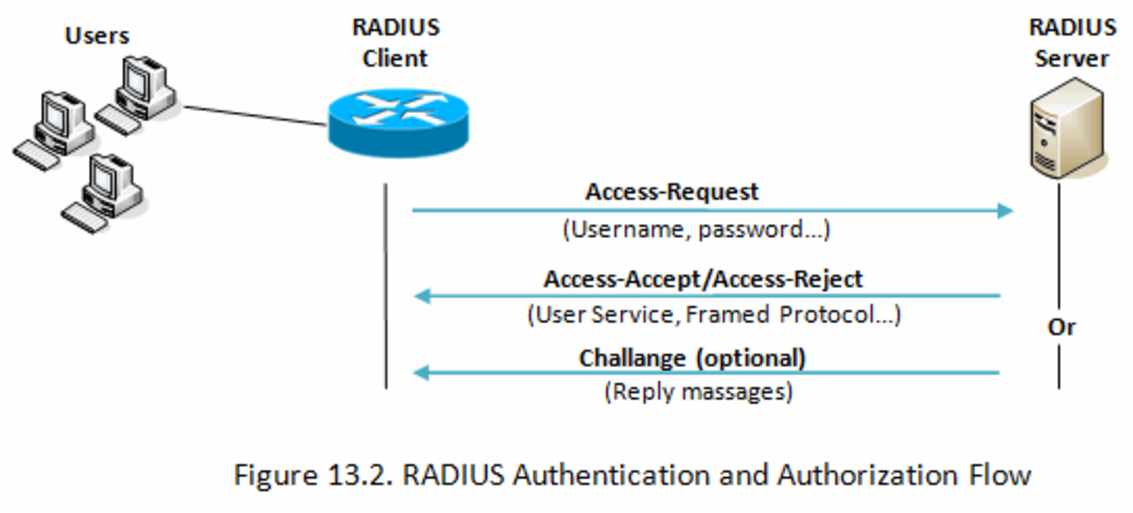
\includegraphics[width=8cm]{figures/Radius}
  \caption{Foobar \cite{einstein}}
\end{figure}


\subsection{Foobar}
Hier kommt alles bezüglich Einleitung MAB foobar
%MAB Cisco Link
%Layer 2 Security Link?
%RADIUS vllt

\section{MAB heutiger Einsatz}
Hier kommt alles bezüglich Einsatz in der heutigen Zeit \cite{Nave:InverseSquareLawSound}
%Fallback
%Drucker, Telefone, IP-Phones, Kameras

\section{Relevanz von MAB in Industrie 4.0}
Hier kommt alles zur Relevanz von Industrie 4.0
%Was ist Industrie 4.0
%Skalierbarkeit, Heterogene Landschaft, Einbindung von "Leichen"

\section{Vor- und Nachteile von MAB}
Hier zählen wir alle vor und Nachteile von MAB auf und kommen danach zum Fazit
Hier würde ich einfach 1 zu 1 die Powerpoint runterschreiben, das haben wir bereits sehr ausführlich gemacht
%Powerpoint verweisen
%Vorteile Nachteile
%Skalierbarkeit vs L2 Security (Spoofing)

\section{Fazit}
Hier kurz was MAB in der Industrie 4.0 für Netzwerke bedeutet und wie es nicht nur als Fallback genutzt werden kann um Netzwerke zu härten.
%Fazit
%Zukunft und Vergangenheit


\bibliographystyle{IEEEtran}
\bibliography{paper}

\end{document}